
\hypertarget{working_projects}{}
\section{Projects}
\index{projects}

\begin{figure}[H]
  \begin{center}
    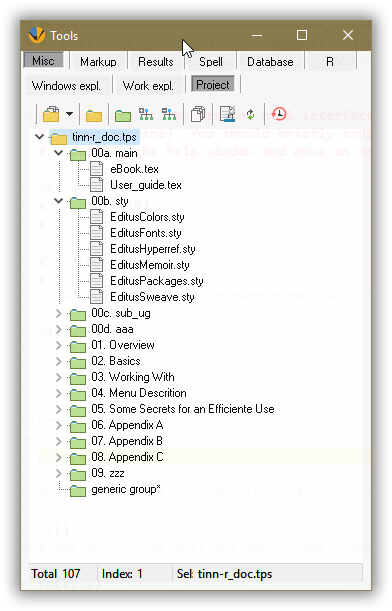
\includegraphics[scale=0.60]{./res/tools_misc_project.png}
  \end{center}
  \caption{Tinn-R: Projects.}
  \label{fig:tinn-r_projects}
\end{figure}

\subsection{Overview}
A Tinn-R project (Figure \ref{fig:tinn-r_projects}) is a container for different types of editable 
files associated with a single task, for example program files, data files, and text files. 
Files in similar categories can be grouped as Tinn-R groups within the project much like folders and subfolders.  
This saves you looking for and opening each of the files individually every time you start working. 
Simply double click on any file in the project or group
(Figure \ref{fig:tinn-r_projects_file_groups})
visible in the \texttt{Tools/Misc/Project} pane
and it will open under a new(s) tab(s) in Tinn-R.

\begin{figure}[H]
  \begin{center}
    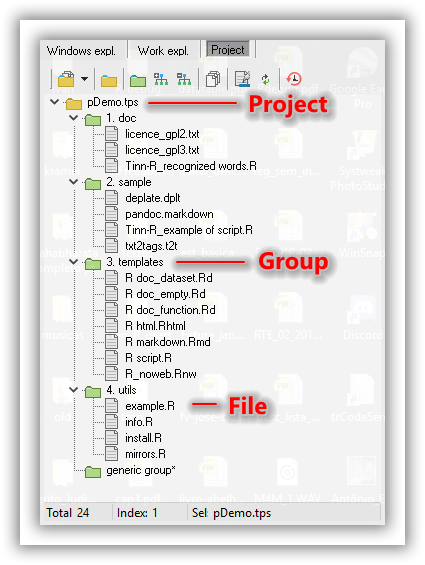
\includegraphics[scale=0.60]{./res/projects_files_groups.png}
  \end{center}
  \caption{Tinn-R: Projects, groups and files.}
  \label{fig:tinn-r_projects_file_groups}
\end{figure}

You can also drag the object (entire project, group or individual file) to the editor. 
Doing so will open the corresponding files for viewing in the editor.

Uneditable files (not ASCII/ANSI/UTF-X, such as PDF, PNG, etc) can be included in 
a project if you will benefit from the listing, but 
they are not correctly viewed in the editor.

\subsection{Opening the demo project}
First, to see a project, you must open the Tools pane: View/Tools/Tools (\texttt{CTRL+F8} by default) 
and choose the page Misc/Project.

You should find a demonstration project (pDemo.tps) at the second (left to right) 
yellow-brown project icon. The option \texttt{Open demo} 
(Figure \ref{fig:tinn-r_projects_open_demo})
will open a didactic demo project. 
You can play around with it to get the general idea.

\begin{figure}[H]
  \begin{center}
    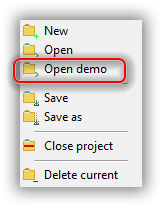
\includegraphics[scale=0.60]{./res/projects_open_demo.png}
  \end{center}
  \caption{Tinn-R: Project demo.}
  \label{fig:tinn-r_projects_open_demo}
\end{figure}

Once you have opened the first project, you can use the first
yellow-brown file-card icon whenever you wish to open a project from the displayed list. 

\subsection{Creating your projects}
To start your own project, click the smaller yellow-brown file-card icon, then \texttt{New}.

The new project will be stored as a \texttt{".tps"} file. Add groups to the project with the green file-card icon.
Add files to a group, or directly to the project itself, with the multiple-sheets icon, then click on \texttt{Add}. 
Files can be selected and dragged and dropped to change the groupings. Groups can be renamed by highlighting 
the group name, then right clicking. Groups can be expanded and contracted all at once with two other icons. 
You can close the Tools pane if it is getting in the way with |X| at the top right.  
Later, re-open it and your project will still be present.

\subsection{Working with the project in graphical mode}
For small projects, changing the project structure is preferable, for example, to add or exclude files, 
change groupings, rename objects directly in graphical mode using the taskbar buttons of the project
and popup menus available. They are self explanatory.

\subsection{Working with the project in text mode}
To create or edit projects with many groups, and/or files, editing in text mode is usually 
more productive than in graphical mode (Figure \ref{fig:tinn-r_projects_text_mode}).

\begin{figure}[H]
  \begin{center}
    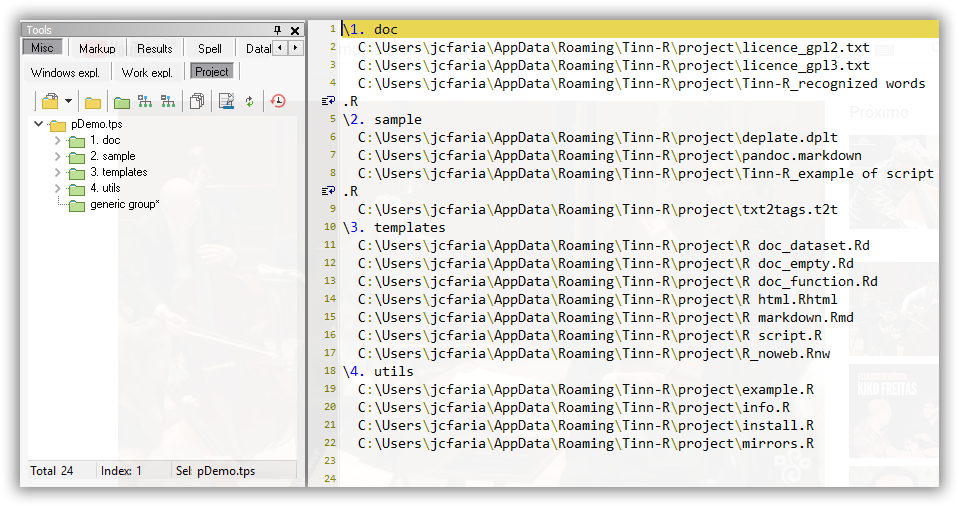
\includegraphics[scale=0.60]{./res/projects_text_mode.png}
  \end{center}
  \caption{Tinn-R: Projects in text mode.}
  \label{fig:tinn-r_projects_text_mode}
\end{figure}

For this, with a project (eg pDemo.tps) open in the GUI, the third button from the right  
on the \texttt{project: edit (as text file)} project taskbar.  This opens the text file in the editor. 
It can then be viewed and edited within the rules for a project file.  
After saving it \texttt{(Crtl+S)}, the second button from left to right will reconstruct the  
graphical interface of the project from its textual description.

\subsection{Submit entire project (or parts) to R interpreter}
If you organize your R scripts into projects with a proper group structure, 
a project popup menu option allows the individual file, group, and entire project to be sent to the interpreter. 
This can be very productive in R package development and more complex data analyses.

\subsection{Sets the main \LaTeX ~project file}
\index{project!sets the main LaTeX project file}
\index{project!main LaTeX project file}
\index{project!LaTeX}
\index{LaTeX}
\index{LaTeX!sets the main LaTeX project file}
\index{LaTeX!main LaTeX project file}
Once you choose a project file as the main one, you can be editing in any project 
file that, when compiling (generate the pdf or dvi), the instruction will be sent correctly
for the compiler. This new feature speeds up the process of creating files (PDF and DVI) 
as the user does not need to navigate to the main file each time to submit the project 
to the compilation. For projects with many files, this feature (already present in more 
specialized \LaTeX ~editors) makes work much easier. The feature is functional for all options
associated with compilation (.pdf, .dvi, makeindex and bibitex). This resource is volatile
with each session and project, that is, it is not stored with the project information.

When there are two main file indications for \LaTeX ~(one in the project and the other in the main
interface for any file), this option, from within the project, takes precedence, that is, it is mandatory.

\subsection{Closing your projects}
When finished with the project, or just to back it up as it is, click the smaller yellow-brown file-card icon, 
then \texttt{Save}.
